\section{مقدمه}
در این تمرین، یک حافظه‌ی نهان (\lr{cache}) سطح \lr{L1} با نگاشت مستقیم (\lr{Direct-Mapped}) با زبان \lr{Verilog} پیاده‌سازی شد. همچنین در بخش دوم تمرین، این \lr{cache} به پردازنده‌ی مشابه \lr{MIPS} (که در تمرین قبل طراحی شده بود) متصل شد.

\section{طراحی حافظه‌ی نهان}

\subsection{ساختار و آدرس‌دهی}
\lr{cache} طراحی‌شده دارای $2^b = 16$ بلاک مستقیم‌نگاشت است ($b=4$) که هر بلاک شامل $2^w = 4$ کلمه‌ی ۳۲ بیتی است ($w=2$)؛ در نتیجه ظرفیت کل کش $2^{b+w} = 64$ کلمه است. آدرس تولیدشده توسط پردازنده سه فیلد دارد:

\begin{table}[H]
    \centering
    \caption{تقسیم‌بندی آدرس ۳۲ بیتی}
    \vspace{0.2cm}
    \begin{tabular}{|c|c|c|c|}
        \hline
        \textbf{بیت‌ها} & \textbf{فیلد} & \textbf{تعداد بیت} & \textbf{کاربرد}                                                 \\
        \hline
        $[31:8]$       & \lr{Tag}      & $c = 24$           & شناسه‌ی بلاک در حافظه‌ی اصلی                                      \\
        \hline
        $[7:4]$        & \lr{Block}    & $b = 4$            & انتخاب یکی از ۱۶ بلاک کش                                        \\
        \hline
        $[3:2]$        & \lr{Word}     & $w = 2$            & انتخاب یکی از ۴ کلمه در بلاک                                    \\
        \hline
        $[1:0]$        & —             & 2                  & \lr{Byte Offset} (همواره صفر؛ دسترسی‌ها \lr{word-aligned} هستند) \\
        \hline
    \end{tabular}
\end{table}

این تقسیم‌بندی با \lr{Bit-Slicing} ترکیبی پیاده‌سازی شده و از هیچ عملیات حسابی استفاده نمی‌کند. آدرس پایه‌ی بلاک با صفر کردن چهار بیت کم‌ارزش محاسبه می‌شود:

\begin{latin}
    \begin{lstlisting}[language=Verilog]
wire [23:0] c_tag   = CPU_Addr[31:8];
wire  [3:0] c_idx   = CPU_Addr[7:4];
wire  [1:0] c_woff  = CPU_Addr[3:2];
wire [31:0] c_baddr = {CPU_Addr[31:4], 4'b0};
wire        hit     = valid[c_idx] && (tag_arr[c_idx] == c_tag);
    \end{lstlisting}
\end{latin}

سیگنال \lr{\code{hit}} به‌صورت ترکیبی محاسبه می‌شود: خط مربوطه باید هم \lr{\code{valid}} باشد و هم \lr{tag} ذخیره‌شده‌اش با \lr{tag} آدرس جاری تطابق داشته باشد. بیت \lr{\code{valid}} برای هر خط مشخص می‌کند که محتوای آن معتبر است یا نه. در ابتدا همه‌ی این بیت‌ها صفر هستند و تنها پس از اولین واکشی از حافظه‌ی اصلی یک می‌شوند. در صورت \lr{hit}، فیلد \lr{\code{c\_woff}} مشخص می‌کند کدام ۳۲ بیت از ۱۲۸ بیت خط به پردازنده برگردانده شود. به عنوان مثال اگر \lr{\code{c\_woff}} برابر صفر باشد، بیت‌های $[31:0]$ خط انتخاب می‌شوند. در غیر این صورت باید از حافظه‌ی اصلی واکشی شود.

\subsection{ماشین حالت}
واسط \lr{cache} از دو بخش تشکیل شده است: از سمت پردازنده، آدرس، نوع دسترسی (خواندن یا نوشتن) و در صورت نوشتن داده‌ی جدید دریافت می‌شود؛ \lr{cache} هم داده‌ی خوانده‌شده و سیگنالی برای اعلام اتمام عملیات (\lr{\code{CPU\_Done}}) به پردازنده برمی‌گرداند. از سمت حافظه‌ی اصلی نیز \lr{cache} می‌تواند درخواست خواندن یا نوشتن یک بلاک 128 بیتی کامل صادر کند و منتظر تأیید (\lr{\code{MM\_Done}}) بماند.

کنترل این بخش با یک \lr{Finite State Machine (FSM)} شش‌حالته مدیریت می‌شود. در یک دسترسیِ خواندن، اگر آدرس در \lr{cache} باشد (\lr{hit})، داده بلافاصله به‌صورت ترکیبی به پردازنده بازگردانده می‌شود و نیازی به تغییر حالت نیست. اگر آدرس در \lr{cache} نباشد (\lr{miss})، ماشین حالت فرایند واکشی از حافظه‌ی اصلی را آغاز می‌کند: درخواست خواندن صادر می‌کند، منتظر پاسخ می‌ماند و پس از دریافت بلاک، آن را در کش نصب می‌کند. در دسترسی نوشتن نیز پس از به‌روزرسانی کش، یک نوشتنِ کامل بلاک به حافظه‌ی اصلی انجام می‌شود.

رفتار دقیق هر حالت به شرح زیر است:

\begin{itemize}
    \item \textbf{\lr{\code{S\_IDLE}}}: این حالت، حالت پیش‌فرض است. در صورت \lr{read hit}، داده‌ی درخواستی مستقیماً از آرایه‌ی \lr{cache} خوانده و به پردازنده بازگردانده می‌شود. در صورت \lr{miss}، ماشین حالت برای واکشی بلاک وارد مرحله‌ی ارسال درخواست به حافظه می‌شود. در صورت \lr{write hit} نیز پس از به‌روزرسانی کلمه‌ی هدف در کش، فرایند نوشتن به حافظه‌ی اصلی آغاز می‌شود.

    \item \textbf{\lr{\code{S\_MM\_RD\_PULSE}}}: درخواست خواندن برای یک چرخه‌ی ساعت به حافظه‌ی اصلی ارسال می‌شود و آدرس بلاک روی خروجی تنظیم می‌شود. ارسال یک‌چرخه‌ای تضمین می‌کند که حافظه‌ی اصلی هر درخواست را دقیقاً یک بار پردازش کند.

    \item \textbf{\lr{\code{S\_MM\_RD\_WAIT}}}: در این حالت ماشین منتظر پاسخ حافظه‌ی اصلی می‌ماند. از آنجا که حافظه‌ی اصلی ممکن است با تأخیر پاسخ دهد، آدرس ارسال‌شده باید تا دریافت تأیید ثابت بماند. پس از فعال شدن \lr{\code{MM\_Done}}، بلاک دریافتی در آرایه‌ی کش نوشته می‌شود؛ اگر درخواست اصلی خواندن بوده به \lr{\code{S\_IDLE}} برمی‌گردد و داده همان چرخه به پردازنده می‌رسد. اگر درخواست نوشتن بوده، کلمه‌ی هدف در بلاک دریافتی جایگزین می‌شود و بلاک به‌روزشده برای نوشتن به حافظه آماده می‌شود.

    \item \textbf{\lr{\code{S\_MM\_WR\_PULSE}}}: درخواست نوشتن برای یک چرخه به حافظه‌ی اصلی ارسال می‌شود. محتوای کامل بلاک به‌روزشده روی \lr{\code{MM\_DataOut}} قرار می‌گیرد.

    \item \textbf{\lr{\code{S\_MM\_WR\_WAIT}}}: مشابه حالت خواندن، آدرس و داده‌ی ارسال‌شده باید تا تأیید حافظه ثابت بمانند، چرا که حافظه‌ی اصلی ممکن است با تأخیر به درخواست پاسخ دهد. با فعال شدن \lr{\code{MM\_Done}}، نوشتن تأیید شده و ماشین وارد حالت بعدی می‌شود.

    \item \textbf{\lr{\code{S\_DONE}}}: نوشتن با موفقیت انجام شده است. در این حالت $\text{\code{CPU\_Done}}=1$ نگه داشته می‌شود تا پردازنده از پایان عملیات مطلع شود؛ به محض اینکه پردازنده این سیگنال را ببیند و درخواست نوشتن را پایین بیاورد، ماشین به \lr{\code{S\_IDLE}} بازمی‌گردد.
\end{itemize}

تمام انتساب‌های رفتاری در بلوک‌های \code{always} با عملگر \code{<=} (\lr{Non-Blocking}) نوشته شده‌اند تا از وقوع \lr{Race Condition} جلوگیری شود.

\subsection{سیاست نوشتن}
سیاست نوشتن در این حافظه، \lr{Write-Through} است. یعنی هر تغییری که در \lr{cache} اعمال می‌شود بلافاصله در حافظه‌ی اصلی هم انجام می‌شود. در \lr{write hit}، تنها 32 بیت مربوط به کلمه‌ی هدف در خط 128 بیتی کش جایگزین می‌شود و بقیه‌ی خط دست‌نخورده می‌ماند؛ سپس بلاک به‌روزشده در حافظه‌ی اصلی نوشته می‌شود. در \lr{write miss} نیز ابتدا بلاک از حافظه‌ی اصلی خوانده می‌شود، کلمه‌ی هدف در آن جایگزین و سپس بلاک کامل در حافظه‌ی اصلی نوشته می‌شود. با این سیاست، محتوای حافظه‌ی اصلی همواره با آخرین وضعیت \lr{cache} همخوانی دارد و نیازی به \lr{Write-Back} در زمان تخلیه‌ی بلاک نیست.

\section{اتصال کش به پردازنده}

\subsection{معماری کلی}
در این بخش، پردازنده و دو نمونه از ماژول کش در یک ماژول بالاسطح (\lr{Wrapper}) کنار هم قرار می‌گیرند. دلیل استفاده از دو کش مجزا این است که جریان دستورات و جریان داده کاملاً از هم مستقلند و نباید یکدیگر را مسدود کنند؛ کش دستور (\lr{icache}) دستور بعدی را واکشی می‌کند در حالی که کش داده (\lr{dcache}) تنها هنگامی فعال می‌شود که دستور جاری نیاز به دسترسی به حافظه دارد.

\lr{icache} همواره در حال خواندن است و آدرس بایتی دستور جاری را به عنوان ورودی دریافت می‌کند. اما \lr{dcache} تنها در دستورات \lr{LW} و \lr{SW} و آن هم فقط پس از اینکه \lr{icache} دستور را تحویل داده باشد فعال می‌شود. این گیت کردن ضروری است، چرا که اگر \lr{dcache} پیش از آماده شدن دستور فعال شود، آدرسی که از دستور ناقص استخراج شده مقدار درستی ندارد و رفتار اشتباه خواهیم داشت.

از آنجا که پردازنده آدرس‌ها را به صورت کلمه‌ای خروجی می‌دهد، اما \lr{cache} ها به آدرس بایتی نیاز دارند، این تبدیل در \lr{Wrapper} انجام می‌شود:
\begin{align*}
    \text{\lr{Byte Address}} = \{\text{\lr{\code{WordAddr[29:0]}}},\ \text{\lr{\code{2'b00}}}\}
\end{align*}

که معادل شیفت دو بیت به چپ است و عملاً همان آدرس بایتی اصلی را بازتولید می‌کند.

\subsection{منطق توقف}
پردازنده یک ورودی توقف خارجی دارد که در صورت فعال بودن، ثبات \lr{PC} ثابت می‌ماند و نوشتن در بانک ثبات هم متوقف می‌شود. این سیگنال زمانی فعال است که حداقل یکی از دو کش هنوز آماده نباشد:
\begin{align*}
    \text{\lr{\code{total\_stall}}} = \lnot\,\text{\lr{\code{icache\_done}}}\ \lor\ \bigl(\text{\lr{\code{dcache\_active}}} \land \lnot\,\text{\lr{\code{data\_done\_flag}}}\bigr)
\end{align*}
\lr{\code{dcache\_active}} زمانی یک است که دستور جاری نیاز به
دسترسی به حافظه‌ی داده داشته باشد (\lr{LW} یا \lr{SW}) و
\lr{icache} هم دستور را تحویل داده باشد. اگر دستور هنوز واکشی نشده باید صبر کرد. اما برای جمله‌ی دوم یک مشکل وجود دارد. پس از اتمام یک دستور \lr{SW}، کش در حالت \lr{\code{S\_DONE}} می‌ماند و $\text{\code{CPU\_Done}}=1$ را نگه می‌دارد تا پردازنده از پایان عملیات مطلع شود. اگر دستور بعدی یک \lr{LW} باشد، \lr{Wrapper} این $\text{\code{CPU\_Done}}=1$ را می‌بیند و آن را به حساب دسترسی \lr{LW} جاری می‌گذارد، در حالی که \lr{dcache} هنوز درخواست جدید را شروع نکرده است.

برای حل این مشکل از یک رجیستر \lr{\code{data\_done\_flag}} استفاده کردیم. این رجیستر هر بار که دستور جدیدی شروع می‌شود (یعنی لحظه‌ای که توقف رفع می‌شود) ریست شده و تنها زمانی 1 می‌شود که \lr{\code{CPU\_Done}} برای دسترسی جاری آمده باشد:

\pagebreak

\begin{latin}
    \begin{lstlisting}[language=Verilog]
always @(posedge Clk or posedge Rst) begin
    if (Rst)
        data_done_flag <= 1'b0;
    else if (!total_stall)
        data_done_flag <= 1'b0;
    else if (dcache_done && dcache_active)
        data_done_flag <= 1'b1;
end
    \end{lstlisting}
\end{latin}

با این روش، \lr{\code{CPU\_Done}} دستورات قبلی روی دستور جاری تأثیر نمی‌گذارد. خروجی \lr{\code{PC}} نیز به طور مستقیم از \lr{\code{InstrAddr}} پردازنده می‌آید و آدرس کلمه‌ای دستور جاری را نشان می‌دهد.

\section{اجرای آزمون}
هر دو بخش را با تست‌بنچ‌های داده شده بررسی کردیم و نتیجه‌ی آنها به این صورت می‌باشد:

\begin{figure}[H]
    \centering
    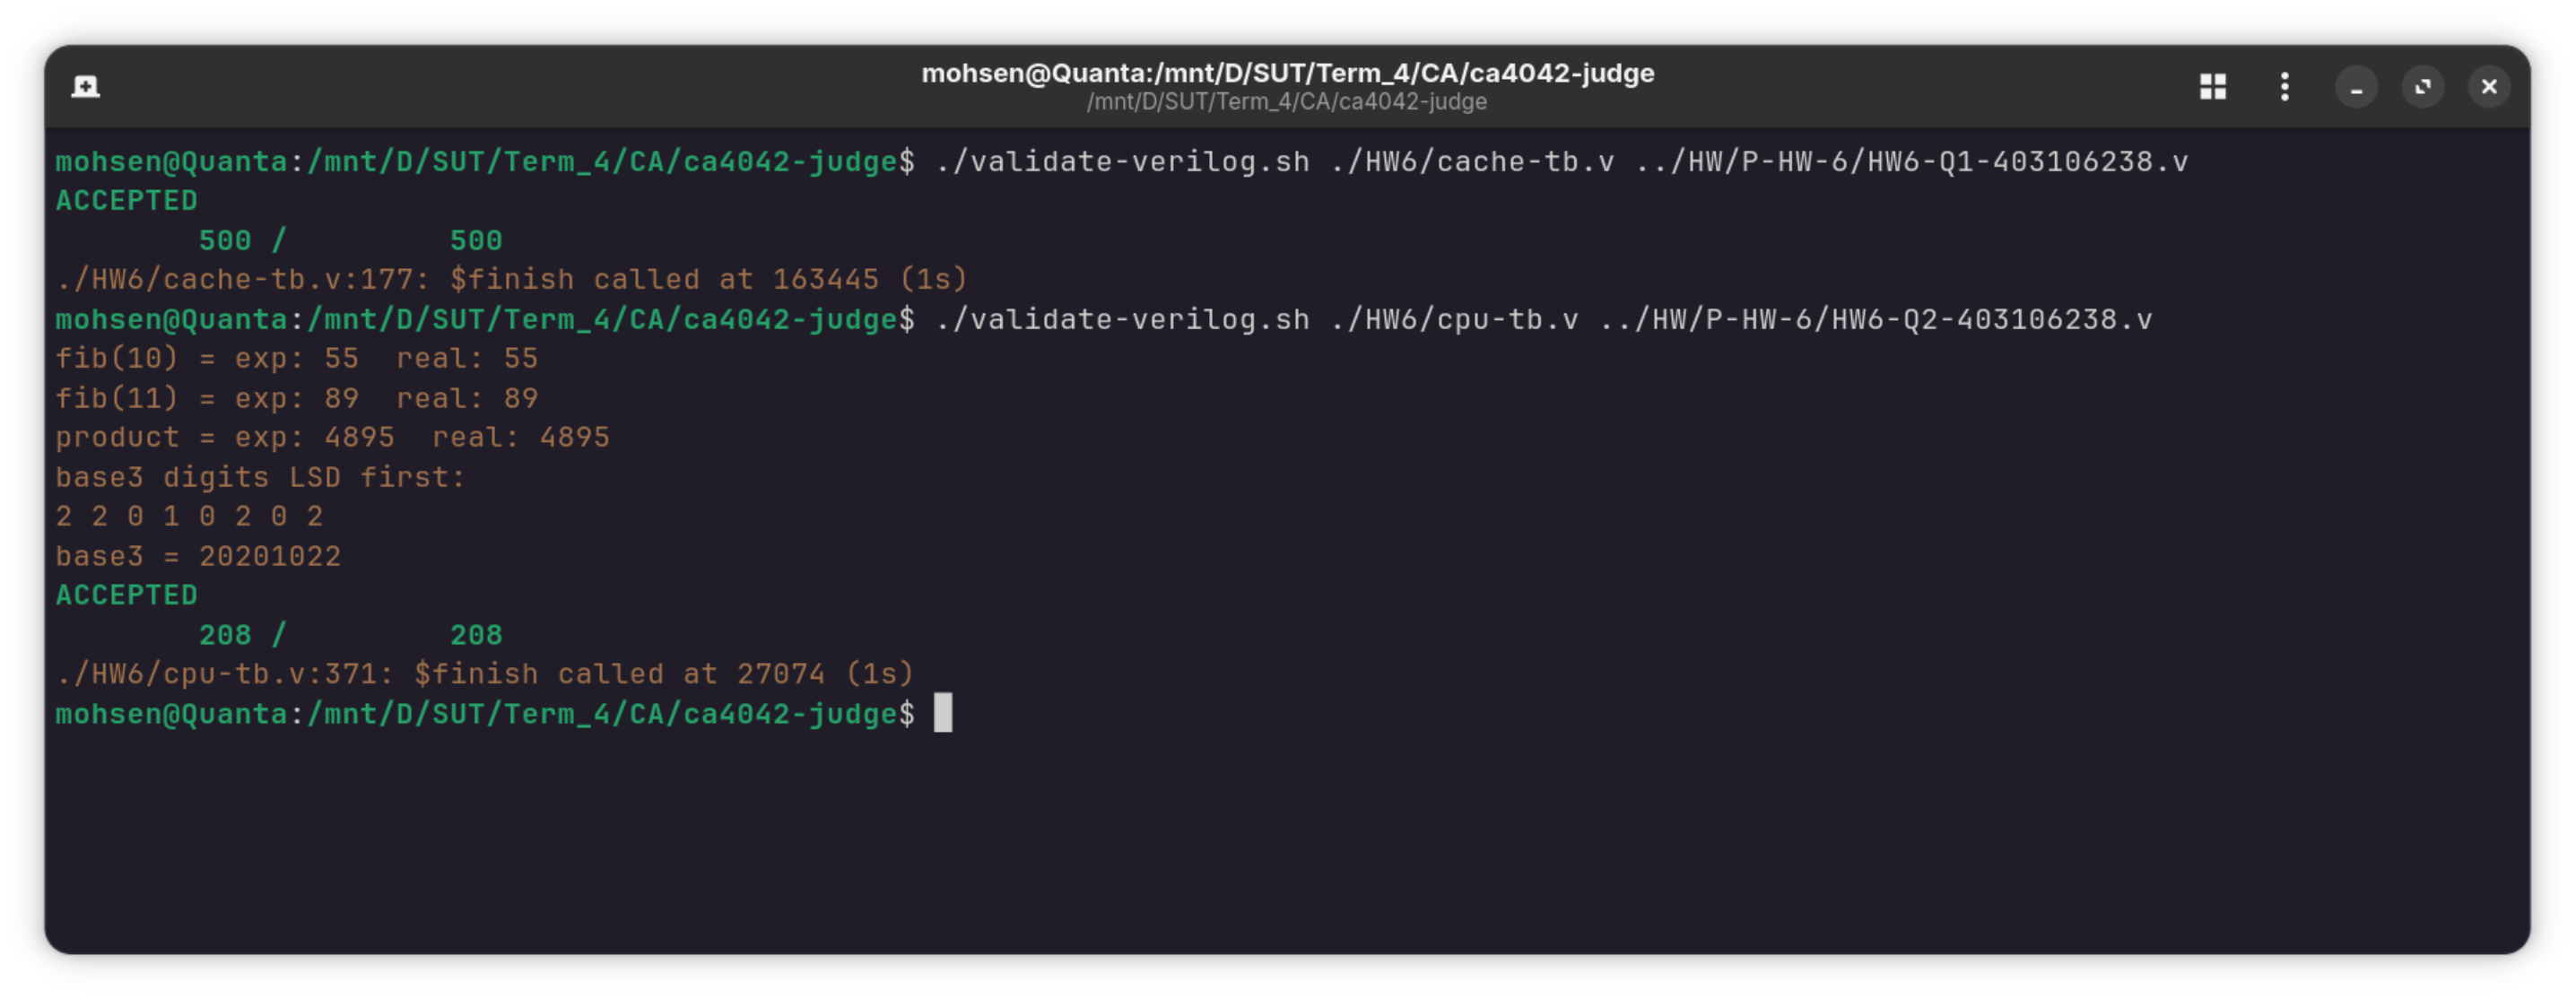
\includegraphics[width=1.0\textwidth]{assets/test_result.png}
    \caption{خروجی آزمون‌های \lr{cache-tb} و \lr{cpu-tb}}
\end{figure}